\documentclass[12pt]{article}

%**********************************************
%* Add additional packages as needed

\usepackage{url,amsmath,setspace,amssymb}
\usepackage{listings}

\usepackage{tcolorbox}
\usepackage{tikz}
\usepackage{xcolor}


\usepackage{color}
\def\R{\color{red}}
\def\B{\color{blue}}

\usepackage[english]{babel}
\usepackage{algorithm}
\usepackage[noend]{algpseudocode}

\usepackage{listings}
\usepackage{caption}
\usepackage{float}
\usepackage{graphicx}
\graphicspath{ {./images/} }

\usepackage{hyperref}


%**********************************************
%* The document starts here
\begin{document}

\tableofcontents

\section{Introduzione}
I problemi di soddifacimento dei vincoli, CSP, e di ottimizzazione, COP, sono spesso problemi difficilmente trattabili (NP-Hard), come nel caso del Vehicle Routing Problem (VRP), o del Job Shop Scheduling (JSS), e allo stesso tempo trovano   
significative applicazioni pratiche, dalla logistica per VRP, all'ottimizzazione dei processi industriali per JSS. 
Questi problemi vengono spesso trattati tramite tecniche di intelligenza artificiale, che possono variare dalla ricerca locale, alla programmazione logica e all'apprendimento per rinforzo \cite{cit:rl}. 

In questo lavoro tratto uno specifico CSP, ‘Fantinew’, la cui soluzione è un piano per il movimento di quattro cavalieri in una scacchiera, sotto ad un insieme di vincoli, con lo scopo di illustrare un linguaggio di programmazione logica, ASP \cite{cit:clingo} e uno di programmazione dei vincoli, Minizinc \cite{cit:minizinc}. 

\section{Problema Fantinew}
\label{sec:problem}
Si consideri una scacchiera di dimensione $n\times n$, dove alcune celle sono occupate ($\text{occ}(x,y)$), altre sono segnate come celle bersaglio ($\text{target}(x,y)$) e le rimanenti sono celle libere. 
Ci sono due input, k, che indica, per ogni cella, il numero massimo di volte che essa può essere visitata, e $t_{max}$, che indica il numero massimo di mosse complessive che possono essere effettuate dai cavalieri. 
Nei quattro angoli della scacchiera sono presenti quattro cavalieri: $A,B,C,D$, che si muovono seguendo le regole della pedina del cavaliere dello scacchi, ovvero possono solo eseguire 
movimenti ad L nella scacchiera, e non possono muoversi al di sopra di un'altro cavaliere. I cavalieri si muovono in ordine, $A,B,C,D,A,B,C,D,\dots$, e non appena un cavaliere non ha più mosse a sua disposizione, il gioco si ferma.

La soluzione del problema è trovare un piano che soddisfi i vincoli enunciati sopra (se esiste), e tale che ogni cavaliere passi almeno una volta su ogni cella bersaglio.


\section{I modelli}
In questa sezione descrivo prima le possibili rappresentazioni delle variabili necessarie alla risoluzione del problema ‘Fantinew’, le loro limitazioni e i vantaggi, poi proseguo spiegando le motivazioni dietro l'
implementazione dei vincoli nei due modelli, partendo dai vincoli che sono espressi allo stesso modo nei modelli Minizinc e Clingo, e proseguendo con le differenze tra i due. 
Infine illustro come interpretare le soluzioni dei due modelli, attraverso un esempio.

\subsection{Modello basato su indici vs modello basato su matrici}
Il problema descritto nella sezione \ref{sec:problem} richiede di far muovere, secondo certi vincoli, quattro cavalieri all'interno di una scacchiera, in una dimensione temporale fissata a $t_{max}$, e quindi 
richiede la modellazione delle celle bersaglio, delle celle occupate, delle posizioni in cui si trovano i cavalieri $A,B,C,D$, in ogni istante di tempo $t$ e del numero di volte in cui ogni cella è stata visitata 
in ogni istante di tempo $t$, ovvero la modellazione di serie temporali di variabili.

Possiamo decidere di rappresentare le serie temporali di variabili sia come una vettore di $t_{max}$ matrici di dimensione $n \times n$, sia come un vettore di $t_{max}$ indici. 
Il modello basato su matrici, rispetto al modello basato su indici, risulta molto informativo, ed è capace di registrare i cambiamenti cumulativi dal tempo $1$ al tempo $t$ in ogni matrice $t$-esima, ma allo 
stesso tempo richiede una quantità di variabili quadratica (sulla grandezza della scacchiera), mentre il modello basato su indici richiede una quantità di variabili costante, ma   
è capace di registrare solamente il cambiamento dal tempo $t-1$, al tempo $t$. 
In generale, se decido di utilizzare il modello ad indice, sono necessarie meno variabili ma più vincoli, e quando decido di utilizzare il modello a matrice, servono meno variabili ma più vincoli. 

Per risolvere il problema ‘Fantinew’ ho implementato due modelli, uno per Minizinc, e uno per Clingo, nei quali rappresento alcune variabili come indici, e altre come matrici, giustificandone la scelta e le limitazioni.

\subsection{Similarità tra i modelli di Minizinc e Clingo}
Il vincolo che esprime il numero massimo di volte in cui una cella può essere visitata è implementato allo stesso modo sia in Minizinc, che in Clingo, attraverso un insieme di $t_{max}$ matrici di dimensione 
$n \times n$, contenenti valori da $0$ a $k$, alle quali è stato imposto un vincolo che, data la matrice $t-1$-esima e la posizione raggiunta dal cavaliere che si è mosso nel tempo $t$, computa la matrice $t$-esima contenente il numero di volte in cui ogni cella è stata visitata nel tempo $t$. 

Una soluzione alternativa sarebbe stata di scartare le matrici delle celle visitate, ed utilizzare al loro posto la rappresentazione a indici delle celle visitate da ogni cavaliere, ovvero, per ogni istante di tempo $t$, di leggere le mosse effettuate dal tempo $1$, fino al tempo $t$ dai cavalieri, in modo da ricostruire, il 
numero di volte in cui ogni cella è stata visitata, ma visto la complessità di questa soluzione, che richiederebbe $O(n^2*t_{max})$ vincoli di tipo ‘count’, ho deciso di optare per la rappresentazione a matrice, la quale, aggiugendo $n^2 * t_{max}$ variabili rispetto al modello a indici, necessita di $O(n^2*t_{max})$ vincoli che controllano che ogni cella al tempo $t$ sia stata visitata $k$ volte al massimo. 
Quindi, utilizzando la rappresentazione a matrici invece che quella ad indici, ho aggiunto delle variabili, mantendendo lo stesso numero di vincoli, ma semplificandone notevolmente la complessità (un vincolo che controlla una disuguaglianza è molto più semplice di un vincolo ‘count’).

Differentemente dal caso delle matrici delle celle visitate, che al costo di un maggiore numero di variabili, riducono considerevolmente la complessità dei vincoli, nel caso del vincolo che verifica che i cavalieri abbiamo visitato tutte le celle bersaglio ad un tempo $t$, 
la maggiore complessità imposta dai vincoli su una rappresentazione a indici è accettabile, considerata la riduzione nel numero delle variabili.
 Per garantire il vincolo, è sufficiente che esista un $t^{'}$, tale per cui tutte le celle bersaglio siano state visitate almeno una volta da ogni cavaliere. Per assicurare questo vincolo, è sufficiente fare quattro test di inclusione tra insiemi, uno per cavaliere, ad ogni istante di tempo $t$, dove si controlla se, 
dato l'insieme delle celle target, espresso come indici, esso sia contenuto nell'insieme delle celle visitate da ogni cavaliere fino al tempo $t$, anch'esso espresso in indici, e quindi, dato che il vincolo di inclusione deve essere eseguito solo $O(t_{max}*4)$ volte, ne giustifico 
l'utilizzo rispetto alla rappresentazione a matrice che, al costo di molte più variabili, garantirebbe solamente una moderata semplificazione dei vincoli.

Un altro vincolo comune tra i due modelli ha come obiettivo costringere le pedine a muoversi come cavalieri dello scacchi, il movimento viene implementato tramite la disgiunzione degli otto movimenti possibili, dei quali almeno uno deve essere eseguito ad ogni tempo $t$.  
Inoltre, sia per Minizinc che per Clingo, si impone nello stesso modo che due cavalieri non possano trovarsi nella stessa posizione al tempo $t$, imponendo un vincolo per ogni combinazione (semplice) di 2 cavalieri, che impedisca che due cavalieri si trovino nella stessa posizione e nello stesso tempo, oltre che un vincolo che 
impedisca ad un cavaliere di spostarsi verso una posizione segnata all'inizio come occupata. 
I vincoli di movimento risultano più complessi per il modello di Clingo, rispetto a Minizinc, perchè, come vedremo nelle differenze tra i due modelli, Clingo necessita di vincoli ulteriori che garantiscano che vengano eseguiti solo movimenti validi.

L'ultimo elemento comune tra i due modelli riguarda il vincolo dell'ordine di movimento dei cavalieri, $A,B,C,D,A,B,C,D,A,B,\dots$. 
Dato che al tempo $t=1$ ogni cavaliere inizia in una posizione prefissata, ovvero $(1,1)$ per A, $(1,n)$ per B, $(n,1)$ per C e $(n,n)$ per D, e che ogni cavaliere si muove solo negli istanti di tempo ad esso assegnati, i quali sono insieme finiti, ovvero A si muove nei tempi $t=2,6,10,\dots$, 
B si muove in $t=3,7,11,\dots$, C in $t=4,8,12,\dots$ e D in $t=5,9,13,\dots$, sia in Minizinc, che in Clingo imponiamo un vincolo che permetta il movimento di un cavaliere solo quando l'istante di tempo $t$ è quello assegnatoli, mentre, quando non tocca a lui, 
aggiorniamo la sua posizione al tempo $t$, copiando quella del tempo $t-1$. Per verificare quale sia il tempo assegnato ad un determinato cavaliere, usiamo la funzione modulo (per esempio, quando $t mod 4 = 2$, allora tocca al cavaliere $A$).

\subsection{Differenze tra i modelli di Minizinc e Clingo}
Una differenza riguarda l'implementazione dei vincoli di movimento dei cavalieri. 
Nel modello di Minizinc è sufficiente imporre il vincolo, per ogni cavaliere, di selezionare una delle 8 mosse possibili, accertandosi di non finire in una posizione occupata, mentre l'implementazione risulta più complicata nel caso del modello Clingo. 

L'implementazione del vincolo di movimento in Clingo prevede che, per ad ognuna delle 8 posizioni raggiungibili dalla posizione $(i,j)$ sia associata un'azione diversa, e che solo un'azione, e una posizione siano selezionabili ad ogni istante $t$, e che quindi, come possiamo vedere nella figura \ref{img:visited_clingo} (sopra), 
se utilizziamo solo le regole di movimento, Clingo potrebbe scegliere un'azione che porta ad una posizione errata, invalidando di conseguenza tutte 8 le scelte valide, e lasciando la libertà a Clingo di scegliere movimenti non validi (per esempio Clingo potrebbe scegliere un'azione che porta fuori dalla scacchiera, invalidando tutti i movimenti validi, e scegliendo una mossa non valida, per esempio spostandosi da $(i,j)$ a $(i+3,j+1)$). 
Per ovviare a questo problema, come possiamo vedere nella figura \ref{img:visited_clingo} (sotto), vengono aggiunte delle regole che impediscono i movimenti invalidi, forzando clingo a scegliere un'azione che corrisponda ad una delle 8 azioni valide. 
\begin{figure}[H]
    \centering
    \includegraphics[width=14cm]{movements_A}
    \caption{Nella figura sopra i vincoli di movimento del cavaliere ‘A’ nel modello Clingo. 
    Sopra sono definiti gli 8 movimenti possibili di un cavaliere, mentre sotto (INERTIA RULES) le regole che forzano a selezionare uno degli 8 movimenti.}
    \label{img:visited_clingo}
\end{figure}

Una soluzione simile viene utilizzata per implementare il vincolo che esprime che il numero massimo in cui una cella può essere visitata è k, forzando il calcolo della $t$-esima matrice delle celle visitate, sulla base della $t-1$-esima matrice, e la cella visitata dal cavaliere che si è mosso al tempo $t$, come si vede in figura \ref{img:movements_A}.
\begin{figure}[H]
    \centering
    \includegraphics[width=14cm]{visited_clingo}
    \caption{Sopra i vincoli per costruire le matrici delle celle visitate, e sotto (INERTIA RULES), il vincolo che forza a costruire le matrici secondo le regole sopra.}
    \label{img:movements_A}
\end{figure}

Una seconda differenza tra i due modelli riguarda le celle bersaglio e le celle occupate, specificate in input nel modello. Nel caso di Clingo, sia le celle bersaglio, che le celle occupate sono espresse sotto forma di indici $(x,y)$, mentre nel caso del modello 
Minizinc, le celle bersaglio sono espresse come dei valori $v \in (1,n^2)$, le quali esprimono univocamente le posizioni di ogni cella della scacchiera di dimensione $n$, e le celle occupate sono rappresentate come una matrice di booleani di dimensione $n \times n$, in 
cui le celle occupate sono impostate a ‘true’.

\subsection{Metodo di ricerca e solver nel modello Minizinc}
Visto che il problema è stato implementato come un insieme di vettori di variabili temporali, che spesso necessitano della variabile calcolata nel tempo $t-1$ per calcolarne il valore nel tempo $t$, 
ho deciso di utilizzare una strategia che selezioni le variabili, all'interno di ogni vettore, in ordine, in modo tale che la variabile $t-1$ venga selezionata prima della variabile $t$, la quale per 
vincolo necessiterebbe comunque del valore della variabile $t-1$ per essere calcolata.

Per quanto riguarda il solver, ho deciso di utilizzare ‘Chuffed 0.10.4’ \cite{cit:solvers}, con l'opzione di ricerca libera, che permette di combinare il tipo di ricerca che abbiamo specificato sopra, con quello 
propria del solver, evitando di utilizzare il solver di default, ‘Gecode’, che dagli esperimenti preliminari dava tempi di esecuzione di un ordine di grandezza superiore, anche su instanze facili del problema.

\subsection{Interpretare le soluzioni}
Le soluzioni di entrambi i modelli vengono fornite come un insieme di indici di posizione per ogni cavaliere, dove sono presenti $t_{max}$ indici, e se la soluzione esiste, allora il modello è soddisfacibile e ritorna una soluzione sotto forma di $t_{max}$ spostamenti, altrimenti è insoddisfacibile. 
Nella figura \ref{img:solution}, espongo la stessa soluzione, sia in Minizinc che in Clingo, di un'istanza di ‘Fantinew’ con $n=8,k=4$ e una singola cella bersaglio di indice $6$, nel quale sono illustrate le posizioni che occupa ogni cavaliere $A,B,C,D$, in ogni istante di tempo $t$, 
e come possiamo vedere, è possibile ricostruire l'intero piano di movimento, da $t=1$, a $t=t_{max}$, di ogni cavaliere, verificando che passi almeno una volta sopra ad ogni cella bersaglio.

\begin{figure}[H]
    \centering
    \includegraphics[width=14cm]{soluzione}
    \caption{Sopra la soluzione in Minizinc, e sotto la soluzione in Clingo, dove sono evidenziate in 4 colori diversi gli istanti di tempo in cui i 4 cavalieri hanno visitato la cella bersaglio numero sei.}
    \label{img:solution}
\end{figure}

\section{Risultati}
Per testare i modelli ho preparato una batteria di 30 istanze del problema ‘Fantinew’, utilizzando il linguaggio R \cite{cit:r}, divise in 3 categorie di difficoltà crescenti. 
Dodici istanze, che sono classificate come facili, variano la grandezza della scacchiera, $n$, da 5 a 7, il valore numero di volte massimo in cui ogni cella può essere visitata, $k$, da 3 a 4 e il numero di celle bersaglio, $v$, da 1 a 2, altre dodici istanze sono classificate di difficoltà ‘media’, con $n \in (12,15)$, $k=4$ e $v \in (2,3)$ celle bersaglio vicine tra loro, e 
infine 6 istanze sono classificate come ‘difficili’, con $n \in (18,20)$, $k=4$ e $v = (3,4)$ celle bersaglio lontane tra loro.

Ho testato le batteria di istanze sia su Clingo, che su Minizinc, e, come possiamo vedere nella figura \ref{img:time_mean}, non solo Minizinc ha un tempo medio di esecuzione considerevolmente inferiore sia nelle istanze medie, che in quelle difficili, ma riesce anche a computare alcune delle ultime prima del tempo limite di 300 secondi, mentre Clingo va sempre in timeout.
Ipotizzo che la differenza in termini di tempi di esecuzione tra le difficoltà media e difficile, per entrambi i modelli, sia dovuta principalmente alla presenza 
di celle bersaglio vicine tra loro nel primo caso, e lontane tra loro nel secondo caso, più che all'aumento della grandezza della scacchiera, 
visto che posizionare celle bersaglio più lontane tra loro aumenta considerevolmente il numero di mosse totali che i cavalieri devono fare per visitarle tutte.
\begin{figure}[H]
    \centering
    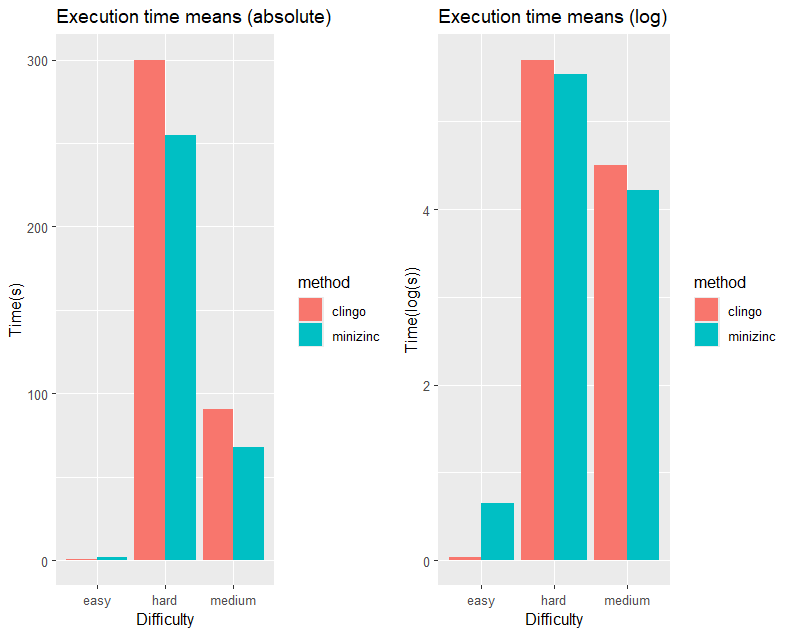
\includegraphics[width=10cm]{time_mean}
    \caption{A sinistra i tempi medi per difficoltà in valore assoluto, mentre a destra il logaritmo degli stessi.}
    \label{img:time_mean}
\end{figure}
Inoltre, come possiamo vedere nella figura \ref{img:time_variance}, anche la varianza dei tempi di esecuzione risulta minore in Minizinc, rispetto a Clingo.
\begin{figure}[H]
    \centering
    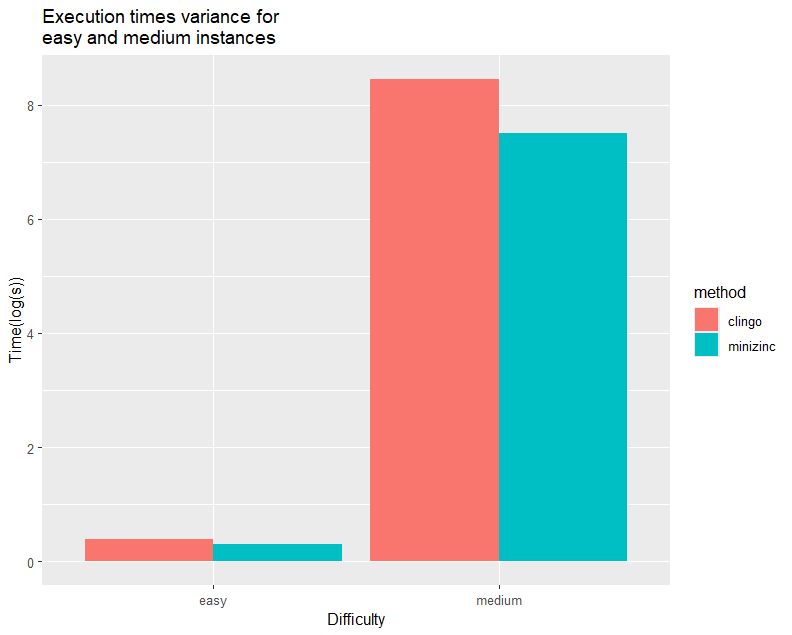
\includegraphics[width=10cm]{time_variance}
    \caption{Sopra la varianza dei tempi di esecuzione per le difficoltà facile e media. La varianza per le istanze difficili non è stata riportata perchè l'esecuzione è andata oltre i 300 secondi per quasi tutte le istanze.}
    \label{img:time_variance}
\end{figure}

\section{Conclusione}
In questo lavoro ho implementato due modelli per la risoluzione del problema ‘Fantinew’, rispettivamente in Minizinc e Clingo. 
I risultati relativi ai tempi medi di esecuzione mostrano che, per il problema in esame, Minizinc con il solver e la strategia di ricerca specificate ottiene, sia in termini di tempi di esecuzione medi, che di varianza dei tempi di esecuzione, valori 
minori rispetto ai tempi di esecuzione ottenuti con il modello di Clingo per tutte le istanze di difficoltà media o superiore.

Inoltre, riporto dai risultati degli esperimenti che il problema non è risolvibile quando il numero massimo di visite per ogni cella, k, è minore o uguale a 3, come suggerito nella descrizione del problema, e questo 
è dovuto al fatto che, visto che ci sono 4 cavalieri, le celle bersaglio devono essere visitate almeno 4 volte.

Un futuro lavoro potrebbe esplorare altri metodi di ricerca per i due modelli proposti in questo lavoro, oppure implementare tecniche diverse dalla programmazione logica, come l'apprendimento per rinforzo combinato con il deep learning \cite{cit:rl}, 
che è già stato applicato con successo a CSP e COP come VRP e JSS \cite{cit:rl_rec}.


\bibliographystyle{IEEEtran}
\bibliography{refs}



\end{document}






